\section{Aktueller Stand}

In diesem Kapitel wird auf den aktuellen Stand der Technik und der Marktintegration von Biogas und Biomethan eingegangen. Zusätzlich wird der rechtliche Rahmen erläutert und Hemmnisse aufgezeigt, die den Prozess hin zu einer Flexibilisierung von Biogasanlagen erschweren.

\subsection{Stand der Technik}

% Je nach eingesetzten Material produzieren die Bakterien Biogas mit einem Methangehalt von 50 bis 75 % https://www.umweltbundesamt.de/themen/wirtschaft-konsum/industriebranchen/biogasanlagen#einfuhrung

\subsection{Stand der Forschung und Entwicklung}

\subsection{Rechtliche Rahmenbedingungen}\label{chap:law_theo}

Grundlage für die Förderung von Biogas- und Biomethananlagen bildet das \gls{EEG}. Das \gls{EEG} wurde erstmal im Jahr 2000 in Kraft gesetzt und enthielt bis einschließlich zur Fassung des \gls{EEG} 2012 hohe Fördersätze für die Erzeugung von Strom aus Biogas. Dies führte zu einem starken Anstieg der installierten Leistung an Biogasanlagen innerhalb dieser Zeitspanne (s. Abb. \ref{fig:ee-cap_biogas}). \parencite{DanielGromke2019}\smallskip

Seither gibt es nur noch einen leichten Zubau an Biogasanlagen, was auf geringere Fördersätze seit dem \gls{EEG} 2014 zurückzuführen ist. Zugleich verschlechterte sich auch für Bestandsanlagen das Umfeld über die sogenannte Höchstbemessungsleistung. Nach \S 101 Abs. 1 ist die \glqq{} Höchstbemessungsleistung [...] die höchste Bemessungsleistung der Anlage in einem Kalenderjahr seit dem Zeitpunkt ihrer Inbetriebnahme und vor dem 1. Januar 2014.\grqq Wobei nach \S 5 Abs. 4 die Bemessungsleistung diejenige Leistung ist, die eine Anlage innerhalb eines Jahres im Durchschnitt erbringt. \parencite{BJV2014a} \smallskip

Die Höchstbemessungsleistung legt fest, bis zu welcher Einspeisung eine Anlage Ihre Vergütung nach dem \gls{EEG} erhält. Liegt die Einspeisung einer Anlage über der Höchstbemessungsleistung, so erhält der Betreiber für jede darüber hinausgehende \si{\kwh} hat somit massiven Einfluss, auf die Erweiterungsfähigkeit von Bestandsanlagen.

\subsubsection{Das Erneuerbare-Energien-Gesetz 2017}



% Hemnisse erläutern
% Warum ab 2014 kein Methanzubau mehr?

\subsection{Stand der Marktintegration von Biogas und -methan}

In diesem Abschnitt wird auf die heutige Rolle von Biogas und -methan in den Sektoren Stromerzeugung, Wärme und Kälte und Verkehr eingegangen. In Tabelle \ref{tab:tab_gas-methane-market} findet sich eine Zusammenfassung der Marktanteile von Biogas und -methan nach Sektoren.

{
\renewcommand{\arraystretch}{1.1}
\begin{table}[H]
	\begin{center}
		\caption{Erzeugung bzw. Endenergieverbrauch aus Biogas und -methan nach Sektoren}
		\begin{tabu} to 0.49\textwidth {X[2] X[r] X[r]}
			\hline
			{}              & Biogas & Biomethan \\
			Sektor          & in \si{\twh} & in \si{\twh} \\ \hline
			Elektrische Energie$^{\mathrm{a}}$ & 29.2  & 2.7      \\
			Wärme und Kälte$^{\mathrm{b}}$     & 13.4  & 3.3      \\
			Verkehr$^{\mathrm{b}}$            & {--} & 6.6       \\ \hline
			\multicolumn{3}{l}{$^{\mathrm{a}}$Erzeugung $^{\mathrm{b}}$Endenergieverbauch } \\
			\multicolumn{3}{l}{Quellen: \parencite{BWE2020}}
		\end{tabu}
		\label{tab:tab_gas-methane-market}
	\end{center}
\end{table}
}

\subsubsection{Stromerzeugung}

Im Jahr 2019 wurden in Deutschland \SI{244.3}{\twh} erneuerbarer Strom produziert, welches einem Anteil von \SI{42.1}{\percent} am Bruttostromverbrauch von \SI{579.8}{\twh} entspricht. Die Bruttostromerzeugung aus Bioenergie stellt mit \SI{50.4}{\twh} einen wesentlichen Anteil an dem produzierten erneuerbaren Strom dar (s. Abb. \ref{fig:ee-gen_total}). \parencite{BWE2020} 

% Bar Chart - EE-Bruttostromerzeugung 2019

\begin{figure}[H]
	\centering
	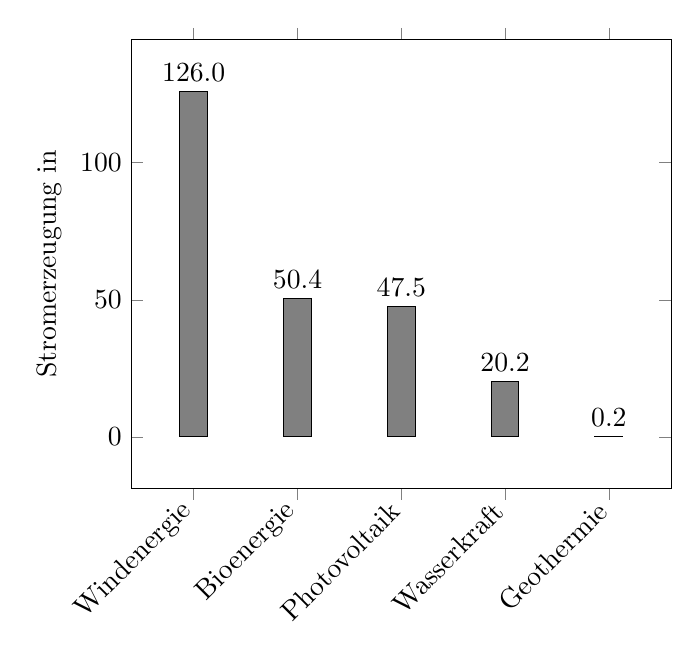
\begin{tikzpicture}
		\begin{axis}[
		ybar,
		enlargelimits=0.15,											% äüßerste bar plots nicht am Limit der x-Achse
		ylabel={Stromerzeugung in \si{\twh}},
		symbolic x coords={Windenergie,
			Bioenergie,
			Photovoltaik,
			Wasserkraft,
			Geothermie 
		},
		xtick=data,
		nodes near coords,											% Zahlen auf den bar plots
		nodes near coords align={vertical},
		nodes near coords style={/pgf/number format/.cd,fixed,fixed zerofill,precision=1},
		x tick label style={rotate=45,anchor=east},
		]
		\addplot[black,fill=black!50!white] coordinates {
			(Windenergie,126.0) (Bioenergie,50.4) (Photovoltaik,47.5) (Wasserkraft,20.2) (Geothermie,0.2)
		};
		\end{axis}
	\end{tikzpicture}
	\caption{Verteilung der Bruttostromerzeugung aus erneuerbaren Energien nach Erzeugungsart im Jahr 2019 \parencite{BWE2020}; \textit{Eigene Darstellung}}
	\label{fig:ee-gen_total}
\end{figure}

Biogasanlagen produzieren mit \SI{29.2}{\twh} den Großteil der Bruttostromerzeugung aus Bioenergie, während Biomethan mit einer Erzeugung von \SI{2.7}{\twh} eine untergeordnete Rolle spielt (s. Abb. \ref{fig:ee-gen_biomass}). \parencite{BWE2020} 

% Bar Chart - Biomasse Bruttostromerzeugung 2019

\begin{figure}[H]
	\centering
	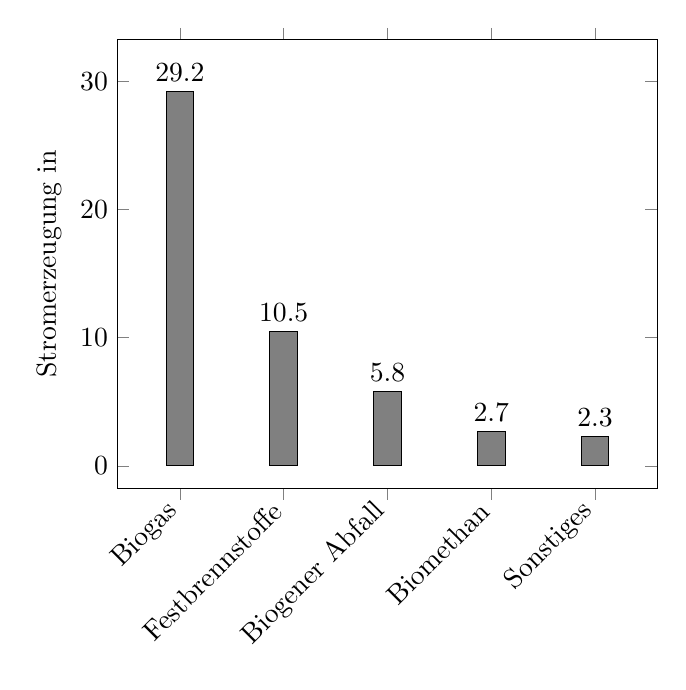
\begin{tikzpicture}
		\begin{axis}[
		ybar,
		enlargelimits=0.15,											% äüßerste bar plots nicht am Limit der x-Achse
		ylabel={Stromerzeugung in \SI{}{\twh}},
		symbolic x coords={Biogas,
			Festbrennstoffe,
			Biogener Abfall,
			Biomethan,
			Sonstiges 
		},
		xtick=data,
		nodes near coords,											% Zahlen auf den bar plots
		nodes near coords align={vertical},
		x tick label style={rotate=45,anchor=east},
		]
		\addplot[black,fill=black!50!white] coordinates {
			(Biogas,29.2) (Festbrennstoffe,10.5) (Biogener Abfall,5.8)
			(Biomethan,2.7) (Sonstiges,2.3)
		};
		\end{axis}
	\end{tikzpicture}
	\caption{Verteilung der Bruttostromerzeugung aus Bioenergie nach Brennstoffart im Jahr 2019 \parencite{BWE2020}; \textit{Eigene Darstellung}}
	\label{fig:ee-gen_biomass}
\end{figure}

Ende 2019 waren in Deutschland mehr als \SI{9000}{\relax} Biogas- und Biomethananlagen mit einer Kraftwerksleistung von \SI{5.9}{\gw} und \SI{0.6}{\gw} am Netz (s. Abb. \ref{fig:ee-cap_biogas}). Seit dem \gls{EEG} 2012 geht der Zubau von Biogasanlagen deutlich langsamer voran als in den vorangegangenen Jahren. Stattdessen erfolgt aufgrund der Einführung der Flexibilitätsprämie in erster Linie eine Erweiterung bestehender Biogasanlagen, um Flexibilität bereitstellen zu können. \parencite{BWE2020} \parencite{DanielGromke2019}

\begin{tikzpicture}
%%% Bar Plot
\begin{axis}[
	ybar stacked,
	ymin=-1500,ymax=7000,
	bar width=10pt,
	legend style={
		at={(0.5,-0.20)},
		anchor=east,
		legend columns=1,
		draw=none},
	legend cell align={left},
	ylabel={Leistung in \si{\giga\watt}},
	symbolic x coords={
		2005,
		2006,
		2007,
		2008,
		2009,
		2010,
		2011,
		2012,
		2013,
		2014,
		2015,
		2016,
		2017,
		2018,
		2019
},
	xtick=data,
	xticklabels={
		2005,,,,,
		2010,,,,,
		2015,,,,
		2019
	},
	%x tick label style={rotate=45,anchor=east},
	ytick={-1000, 0, 1000, 2000, 3000, 4000, 5000, 6000},
	yticklabels={, 0,, 2,, 4,, 6}
	]
\addplot+[ybar, draw=black, pattern=north east lines] plot coordinates {(2005,665) (2006,1000) (2007,1226) (2008,1419) (2009,2520) (2010,3015) (2011,3837) (2012,4212) (2013,4317) (2014,4380) (2015,4601) (2016,4780) (2017,5173) (2018,5597) (2019,5901) };
\addplot+[ybar, draw=black, fill=black!50!white] plot coordinates {(2005,0) (2006,0) (2007,6) (2008,16) (2009,18) (2010,96) (2011,218) (2012,256) (2013,383) (2014,603) (2015,614) (2016,653) (2017,567) (2018,557) (2019,558) };
\legend{\strut Inst. Leistung Biogas, \strut Inst. Leistung Biomethan}
\end{axis}

%%% Line Plot
\begin{axis}[
	ymin=-150,ymax=700,
	axis y line*=right,
	legend style={
		at={(0.5,-0.20)},
		anchor=west,
		legend columns=1,
		draw=none},
	legend cell align={left},
	ylabel={Zubau in \si{\mega\watt}},
	symbolic x coords={
		2005,
		2006,
		2007,
		2008,
		2009,
		2010,
		2011,
		2012,
		2013,
		2014,
		2015,
		2016,
		2017,
		2018,
		2019
},
	xtick=data,
	xticklabels={,,,,,,,,,,,,,,,,,,,,,,,,,,,,,},
	ytick={-100, 0, 100, 200, 300, 400, 500, 600},
	yticklabels={, 0,, 200,, 400,, 600}
	]
\addplot[sharp plot, draw=black, very thick] plot coordinates {(2005,0) (2006,0) (2007,6) (2008,10) (2009,2) (2010,78) (2011,122) (2012,38) (2013,127) (2014,220) (2015,11) (2016,39) (2017,-86) (2018,-10) (2019,1)};
\legend{\strut Nettozubau Biomethan}
\end{axis}
\end{tikzpicture}

In den Jahren 2010 bis 2014 gibt es einen verstärkten Ausbau von Biomethananlagen. Ab dem \gls{EEG} 2014 (s. Kap. \ref{chap:law_theo}) kommt es zu einem starken Einbruch in dem Zubau von Kraftwerksleistung und in den Jahren 2017 und 2018 ist dieser mit einem Rückbau von \SI{86}{\mw} bzw. \SI{10}{\mw} sogar negativ (s. Abb. \ref{fig:ee-cap_biogas}). Hier zeigt sich die Abschwächung der Anreize seit Neuauflage des \gls{EEG} 2014. \parencite{BWE2020} \smallskip

Insgesamt bedeutet dies, das ein Großteil der bestehenden Anlagenleistung innerhalb des nächsten Jahrzehnts seine Förderung nach dem \gls{EEG} verlieren wird. Es ist somit dringend geboten alternative Erlösströme zu finden, die über dem Niveau einer reinen Direktvermarktung an der Strombörse liegen. Da das niedrige Preisniveau der Strommarkterlöse ansonsten zu einem Rückgang der Stromerzeugung aus Biogasanlagen führen würde. Deshalb soll diese Arbeit aufzeigen, ob die Biogasaufbereitung zu Biomethan eine solche Möglichkeit darstellen kann.

% Wie viel kann man an der Strombörse verdienen?

\subsubsection{Wärme und Kälte}

Der Endenergieverbrauch in dem Sektor Wärme und Kälte entsprach im Jahr 2019 \SI{13.4}{\twh} an Biogas und \SI{3.3}{\twh} an Biomethan. Dies entspricht einem Anteil von \SI{1.1}{\percent} bzw. \SI{0.3}{\percent} an dem Gesamtendenergieverbrauch in der Erzeugung von Wärme und Kälte von \SI{1216.7}{\twh}. Ein Großteil der erneuerbaren Wärmeerzeugung von insgesamt \SI{152.0}{\twh} aus Bioenergie stammen hingegen aus Festbrennstoffen. \parencite{BWE2020}\smallskip

Es ist davon auszugehen, dass der Einsatz von Biomethan in Zukunft zunehmen wird. Vor allem kann Biomethan eine stärke Rolle in der Erbringung von industrieller Prozesswärme bei hohen Temperaturen und bei der Spitzenlastdeckung übernehmen. Insgesamt wird ein Einsatz von \SI{18}{\twh} bis \SI{35}{\twh} an Biomethan an der Wärme- und Kälteproduktion im Jahr 2050 prognostiziert. \parencite{dena2017}

\subsubsection{Verkehr}

Mit einem Endenergieverbrauch von \SI{0.7}{\twh} an Biomethan und einer gesamten Erzeugung aus erneuerbaren Energie von \SI{36.9}{\twh} im Verkehrssektor im Jahr 2019 ist der Anteil am Gesamtmarkt von \SI{656.8}{\twh} sehr gering. \parencite{BWE2020} \smallskip

Zukünftig kann Biomethan in Form von Bio-\gls{LNG} im \mbox{Schwerlast-,} Schiffs- und Flugverkehr eine bedeutendere Rolle übernehmen. Da in diesem Bereich voraussichtlich Verbrennungsmotoren für lange Zeit die dominierende Antriebstechnologie bleiben werden. \parencite{dena2017}